\documentclass{article}
\usepackage{graphicx}
\usepackage{float}
\usepackage{gensymb}
\parskip=12pt

\begin{document}

\title{Laboratory 5: Geometric Optics}
\date{December 3, 2014}
\author{Calvin Chan\\304144970\\Physics 4BL Lab 8\\Partners: Caleb Choi, Stanley
Chan}

\maketitle

\section{Introduction}

This lab aims to demonstrate various optical theories. By sending a ray through
a trapezoidal prism, we can observe the incident and refracted angles of the
ray, thus calculating the theoretical value of the index of refraction. We can
then verify Snell's law by physically finding the critical angle of the prism to
see how the experimental and theoretical values of the index of refraction
compare.

Following that, We measure the focal lengths of three lenses biconcave,
plano-convex, and biconvex. We can shine rays through the lenses and observe
where the rays converge, whether it's before or after the lens. By isolating and
removing certain rays, we can observe the effects of spherical aberration.
Additionally, we can observe the effects of magnification through the biconcave
and biconvex lenses by measuring the distance between the rays before and after
the rays are refracted. Finally, we can shine the rays through thin lenses and
observe where the rays converge (focal length). This final experiment can be
used to verify the equation of a combination of lenses and the image-object
equation.

\section{Experimental Results}

\subsection{Snell's Law and Total Internal Reflection}

A monochromatic ray of light was shot into a trapezoidal prism as shown in
figure \ref{trapezoidal_prism}. We measured the incident and transmitted angles
of the ray (both measured against the normal of the front interface)
to be $33\degree$ (0.576 rad) and $19\degree$ (0.332 rad), respectively.

\begin{figure}[H]
    \centering
    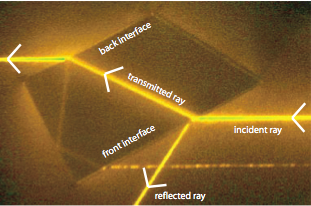
\includegraphics[width=0.7\textwidth]{charts/trapezoidal_prism}
    \caption{The trapezoidal prism}
    \label{trapezoidal_prism}
\end{figure}

We measured then measured the angles of the ray as it exited the prism through
the back interface. Inside the prism, it approached the back interface at an
angle of $18 \degree$ (0.314 rad) to the normal, and exited with an angle of $32
\degree$ (0.559 rad) to the normal.

We then used a similar method to find the critical angle for the prism – the
angle of incidence at which there is no refraction, but just total internal
reflection inside the prism. We measured the incident angle of ray to the front
interface to be $27 \degree$ (0.471 rad) and the angle of the transmitted ray
inside the prism to be $16 \degree$ (0.279 rad). The critical angle inside the
prism was measured to be $44 \degree$ (0.768 rad), the incident angle as the ray
approached the edge from within the prism itself.

\subsection{Thick Lenses}

\begin{figure}[H]
    \centering
    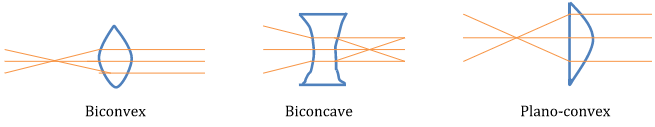
\includegraphics[width=\textwidth]{charts/thick_lenses}
    \caption{Using the ray box, light rays were shined into various thick lenses
    from the right to observe their focal lengths}
    \label{thick_lenses}
\end{figure}

For this section of the lab, we measured the focal lengths of various thick
lenses: biconcave, biconvex, and plano-convex (ref. figure \ref{thick_lenses}).
For the biconcave lens, we used the ray box to shine three rays at the lens,
tracing the diverging rays back to one point before the lens. We then measured
the distance between the lens and the point to be $30.5mm$, the focal length of
the biconcave lens. Similarly, we shined three rays at the biconvex lens and the
rays converged on the other side of the lens, a distance of  $58mm$ away from
the lens. We performed the same process on plano-convex lens, and recorded the
convergence of the rays at a distance of $94mm$ away from the lens. The
following chart shows the focal lengths of all the thick lenses. 

\begin{figure}[H]
    \centering
    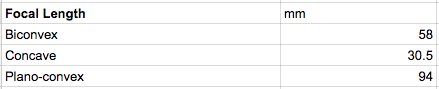
\includegraphics[width=0.7\textwidth]{charts/thick_lenses_focal_length}
    \caption{Focal lengths for various thick lenses}
    \label{thick_lenses_focal_length}
\end{figure}

\begin{figure}[H]
    \centering
    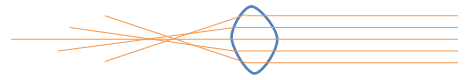
\includegraphics[width=0.7\textwidth]{charts/spherical_aberration}
    \caption{Spherical aberration exhibited by the biconvex lens}
    \label{spherical_aberration}
\end{figure}

Next, we used the ray box to shine 5 parallel rays of light into a biconvex
lens (figure \ref{spherical_aberration}). We could observe the effects of
spherical aberration through the rays near the edge of the lens, as they
effectively had a different focal point than the three inner rays. We measured
the positions of both focal points and determined the distance between them, as
shown in the following chart.

\begin{figure}[H]
    \centering
    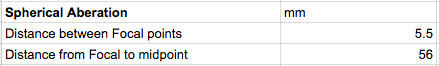
\includegraphics[width=0.7\textwidth]{charts/thick_lenses_spherical_aberration}
    \caption{Distances between focal points due to spherical aberration}
    \label{thick_lenses_spherical_aberration}
\end{figure}

\begin{figure}[H]
    \centering
    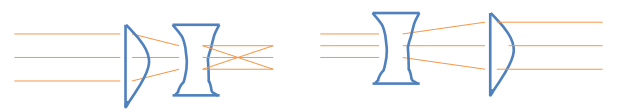
\includegraphics[width=0.7\textwidth]{charts/magnification}
    \caption{Combining two lenses to experiment with magnification and
    demagnification}
    \label{magnification}
\end{figure}

Finally, we used both, the biconvex lens and the biconcave lens together to observe
magnification properties of the lenses (figure \ref{magnification}). Using the
ray box, we shined three rays of light into the biconvex lens followed by a
biconcave lens to demonstrate demagnification. We then switched the order of the
lenses (biconcave followed by biconvex) and experimented with various distances
between the lens and ray box to find the maximum magnification. We measured the
distances between the rays before and after the magnification and
demagnification, as shown in the following chart.

\begin{figure}[H]
    \centering
    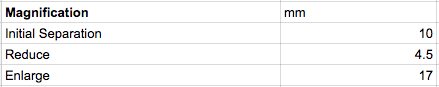
\includegraphics[width=0.7\textwidth]{charts/thick_lenses_magnification}
    \caption{Magnification through biconvex and biconcave lenses}
    \label{thick_lenses_magnification}
\end{figure}

\section{Analysis}

\begin{equation}
    \label{vflambda}
    v = f\lambda
\end{equation}
\begin{equation}
    \label{vflambda_sound1}
    v = (6.6kHz)(2\cdot0.0244)
\end{equation}
\begin{equation}
    \label{vflambda_sound2}
    v = 351.35 \frac{m}{s}
\end{equation}

\section{Conclusion}
This experiment successfully demonstrated properties of sound waves and light
waves. We successfully calculated the speed of sound within the uncertainties
and errors that propogated through the experiment using the relationship between
angular frequency and wave vector. Furthermore, our calculations using the
standing waves for both sound and light were close to the actual values of the
speeds of sound and light, with errors falling within the threshold yielded
by error propogation.
\end{document}
